\documentclass{article} % For LaTeX2e
\usepackage{nips15submit_e,times}
%\usepackage{hyperref}
\usepackage{url}

\usepackage{subfigure}
\usepackage[margin=1in]{geometry}
\usepackage{amsmath, amsfonts}
\usepackage{enumerate}
\usepackage{graphicx}
\usepackage{url}
\usepackage{xcolor}
\usepackage[colorlinks=true,urlcolor=blue]{hyperref}
\usepackage{bbm}
\usepackage{float}

%\documentstyle[nips14submit_09,times,art10]{article} % For LaTeX 2.09


\title{Final Report: Predicting student's learning performance with KDD Cup 2010}


\author{
Binbin Xiong\\
Information Networking Institute\\
Carnegie Mellon University\\
Pittsburgh, PA 15213 \\
\texttt{bxiong@andrew.cmu.edu} \\
\And
Yujing Zhang\\
Information Networking Institute\\
Carnegie Mellon University\\
Pittsburgh, PA 15213 \\
\texttt{yujingz1@andrew.cmu.edu}
}

% The \author macro works with any number of authors. There are two commands
% used to separate the names and addresses of multiple authors: \And and \AND.
%
% Using \And between authors leaves it to \LaTeX{} to determine where to break
% the lines. Using \AND forces a linebreak at that point. So, if \LaTeX{}
% puts 3 of 4 authors names on the first line, and the last on the second
% line, try using \AND instead of \And before the third author name.

\newcommand{\fix}{\marginpar{FIX}}
\newcommand{\new}{\marginpar{NEW}}

\nipsfinalcopy % Uncomment for camera-ready version

\begin{document}

\maketitle

\begin{abstract}
KDD Cup 2010 is an educational data mining problem of practical importance. It is to learn a model from students' past behavior and then predict their future performance. We extracted five features: \emph{student ID}, \emph{problem name}, \emph{step}, \emph{knowledge component}, and \emph{opportunity count} from the dataset to predict the binary value of \emph{correct first attempt}. Then, we implemented several classifiers including Naive Bayes, Logistic Regression, and SVM as our training models. In addition, we used Adaboost and k-means these two techniques to optimize the training process. At last, we compared each classifier with accuracy and Root Mean Squared Error to analyze the results.

\end{abstract}

\section{Background}
What is a student's learning generality and speed? What is the difference and similarity between problems How can we the difficulty degree of a problem? These problems might be solved by analyzing the knowledge concepts and skills each problem needs.


\subsection{Problem Description}

In this report, we are tackling the problem of student learning process. We predict the student learning performance on mathematical problems given information regarding past performance, with the 2010 Knowledge Discovery and Data Mining competition dataset. This problem is not only a technical topic for researchers, but also of practical importance.

%% \subsection{Double-blind reviewing}

%% This year we are doing double-blind reviewing: the reviewers will not know 
%% who the authors of the paper are. For submission, the NIPS style file will 
%% automatically anonymize the author list at the beginning of the paper.

%% Please write your paper in such a way to preserve anonymity. Refer to
%% previous work by the author(s) in the third person, rather than first
%% person. Do not provide Web links to supporting material at an identifiable
%% web site.

%%\subsection{Electronic submission}
%%
%% \textbf{THE SUBMISSION DEADLINE IS June 5, 2015. SUBMISSIONS MUST BE LOGGED BY
%% 23:00, June 5, 2015, UNIVERSAL TIME}

%% You must enter your submission in the electronic submission form available at
%% the NIPS website listed above. You will be asked to enter paper title, name of
%% all authors, keyword(s), and data about the contact
%% author (name, full address, telephone, fax, and email). You will need to
%% upload an electronic (postscript or pdf) version of your paper.

%% You can upload more than one version of your paper, until the
%% submission deadline. We strongly recommended uploading your paper in
%% advance of the deadline, so you can avoid last-minute server congestion.
%%
%% Note that your submission is only valid if you get an e-mail
%% confirmation from the server. If you do not get such an e-mail, please
%% try uploading again. 


\subsection{KDD 2010 Data Set Description}

The dataset is divided into a training set and a test set. Four key terms form the building blocks of the dataset. These are problem, step, knowledge component, and opportunity. A problem is a task for a student to perform, and it typically involves multiple steps, which are observable parts of the solution to a problem. A knowledge component is a piece of information that is used to solve a step. It can be concept, principle, fact, skill, etc. Each step can be labeled with one or more hypothesized knowledge components. And every knowledge component is associated with one or more steps. Finally, an opportunity is a chance for a student to demonstrate whether he or she has learned a given knowledge component. In this report, we predict the binary value of "correct first attempt'' as student-step performance.

\section{Related Works}
\label{gen_inst}

In[2], the authors points out that feature extraction is playing a vital role in this problem. In addition, as the student is learning during the tutoring process, temporal information is of great importance. Their work can be separated into two parts: feature extraction and classification. 
For feature extraction, they use two techniques: sparse features generated by expanding a multi-category feature into a set of binary features, and condensed features using feature combinations to indicate some relationships. For classification part, they tried several machine learning techniques to train the learner. They use Logistic Regression for sparse feature set, and use Random Forest, AdaBoost for dense feature set. Finally, they combined all results from different classifiers by regularized linear regression, and won the first place of the competition.

The final prediction of the 2nd team[3] was a combination of Bayesian Hidden Markov Models (HMMs) and bagged decision tree.Their HMM model learns student specific parameters and then used them to train skill specific models. It was to predict the probability of knowledge for each student at each opportunity and the probability of correctness on each step. Then they used the prior skill data learned to generate features for the test sets, and implemented Random Forest to do the prediction.

The team of 3rd place[4] used Singular Value Decomposition (SVD) technique, and won the third place. Based on the idea of SVD model, they tried several factor models in order to correct the shortcomings of pure SVD. They introduced many biases into the model, like a step dependent bias, a student dependent bias, a KC dependent bias, a student and KC dependent bias, etc. In addition, they used KC dependent N dimensional feature vectors. Both of the bias and feature vector methods significantly lowered the value of RMSE.



%The version of the paper submitted for review should have ``Anonymous Author(s)'' as the author of the paper.

\section{Learning Model}
According to implicit relationship among data fields, we extract several key features and build a feature model. Then we use both discriminative and generative models including Naive Bayes, Logistic Regression, and SVM to learn and test the \emph{Algebra I 2005-2006} data set. In order to improve learning performance, we implement  two techniques: AdaBoost and k-means, to obtain a higher classification accuracy as well as a lower rooted mean squared error.

\subsection{Feature Extraction}
There are 19 columns in total in the dataset, but some of them are irrelevant to our prediction, like row number. We extract some important features to build the learning model. Different problems and knowledge components have different difficulty degrees. Some are easy to solve, but others are hard. In addition, the more times a knowledge component the student meet, the easier the step for the student. And different students have different learning rate. So we decide to use \emph{student ID}, \emph{problem name}, \emph{step}, \emph{knowledge component}, and \emph{opportunity count}  as five features of our learning model. In addition, we use the value of \emph{corret first attempt} as student-step performance predictor.

\subsection{Naive Bayes}
Naive Bayes classifier is a simple probabilistic classifier based on applying Bayes Theorem with conditional independent given class label. Assume $X=\{ x_1, x_2,..., x_n\}$ is a collection of features, and $Y=\{1,0\}$. Each $x_i$ is a discrete feature, and $x_i\in X$ is independent given Y. Then: 

\begin{equation}
\begin{aligned}
P(Y=y \mid x_1, x_2,..., x_n)=\frac{P(Y=y) \prod_{i=1}^{n} P(x_i \mid Y=y))}{\sum_{k=0}^{1} P(Y=k)\prod_{i=1}^{n} P(x_i \mid Y=k)}\\
Y\leftarrow \arg\max_{y_k} P(Y=y_k) \prod_{i=1}^{n} P(x_i \mid Y=y_k) 
\end{aligned}
\end{equation}
Naive Bayes classifier can be trained in linear time, rather than by expensive iterative approximation as used for many other types of classifiers. Applying MAP estimation in Naive Bayes is necessary to avoid overfitting and extreme probability values. 

\subsection{Logistic Regression}
Logistic Regression is also a probabilistic statistical classification model. For binary classification: 

\begin{equation}
\begin{aligned}
P(Y=1\mid X)=\frac{1}{1+exp(w_0+\sum_{i=1}^{n} w_iX_i)} ~~~~~ P(Y=0\mid X)=\frac{exp(w_0+\sum_{i=1}^{n} w_iX_i)}{1+exp(w_0+\sum_{i=1}^{n} w_iX_i)} 
\end{aligned}
\end{equation}

This problem can be solved through gradient ascent, which is to update the vector of parameters iteratively, until it satisfies some termination condition. In addition, to reduce overfitting, Logistic Regression is allowed to add a regularization term $P(W)$. In our implementation, we plan to use both L1 and L2 norm, which can be represented as:
\begin{equation}
\begin{aligned}
L1: \ln P(W) \propto \sum_i \mid w_i \mid && L2: \ln P(W) \propto \sum_i w^2_i
\end{aligned}
\end{equation}
Compared to Naive Bayes, Logistic Regression has no assumption that features are independent with each other conditional on label, but it can only produce a linear decision boundary.


\subsection{Support Vector Machine}
Support Vector Machine (SVM) is a discriminative classifier formally defined by a separating hyperplane. In other words, given labeled training data (supervised learning), the algorithm outputs an optimal hyperplane that gives the maximum margin $\gamma$ to the training examples.
\begin{equation}
\begin{aligned}
&\underset{w}{\min}&&||w||^2_2 + C\sum\limits_{i=1}^m\xi_i\\
&\text{subject to } &&y_i(w^{T_i}x_i) \geq 1-\xi_i &\forall i\\
&&&\xi_i\geq 0 &\forall i
\end{aligned}
\end{equation}
Here the \emph{C} is the slack variant that we need to assign before starting the training process.

The goal of SVM is to find a linear boundary with the maximum margin of the different labels. Therefore, if the data is linearly separable, the \emph{linear} boundary that the SVM finds should be with a rather high accuracy. With the same cost function shown above, in addition to performing linear classification, SVMs can efficiently perform a non-linear classification using the \emph{kernel trick}, which can implicitly mapping their inputs into high-dimensional feature spaces. A typical kernel function that can map the feature into a infinite space is the Gaussian kernel (which is also known as RBF), which can be represented as:

\begin{equation}
\begin{aligned}
&K(X_i, X_j) = \exp (- \gamma ||X_i - X_j||^2), \text{for } \gamma > 0
\end{aligned}
\end{equation}

Thus if we train a non-linear classifier, even if the training data is not linear separable, it should still give a rather decent accuracy, which means that by applying both linear and none-linear SVM classifiers, the change of the accuracy of them \emph{should} tell us something of the distribution of training data. Therefore, we may implement both linear and none-linear with RBF kernel L1 SVM classifiers in our system.  

\subsection{AdaBoost}
AdaBoost is adaptive boosting algorithm. It can turn weak algorithm into a strong learner by concentrating on examples misclassified by previous iteration and combining hypothesis of each iteration as the final hypothesis. 

For dataset $S=\{(x_1, y_1),...,(x_m, y_m)\}; x_i\in X, y_i\in Y=\{-1, 1\}$ and weak algorithm A, construct example distribution $D_t (t=1,2,...T)$. 
$$D_{t+1}=\frac{D_t(i)}{Z_t}\exp\{-\alpha_i y_i h_t(x_i)\} ~~~~(D_1=\frac{1}{m})$$
Run A on $D_t$ producing $h_t$:
$X\rightarrow \{-1, 1\}, \epsilon_t=P_{x_i}(h_t(x_i)\ne y_i)$
$$\alpha_t = \frac{1}{2}\ln{\frac{1-\epsilon_t}{\epsilon_t}}$$
$$H_final(x)=sign(\sum_t {\alpha_t h_t(x)})$$

AdaBoost can be used to improve the learning performance for any weak algorithms, like Naive bayes, decision stumps, etc. It converges vary fast, and has no parameters to tune. In addition, when training accuracy converges, the test accuracy could be further improved as the number of rounds increasing.

\subsection{K-Means}
K-Means is an unsupervised learning algorithm. It partitions data into k clusters with the nearest distance to the cluster center(mean). Assume that $d(x, y)$ represents the distance between point x and y. The algorithm aims to find center $c_1, c_2, ..., c_k$ of k clusters, and
$$minimize \sum_{i=1}^{n}{min_{j\in\{1, 2, ..., k\}} d^2(x_i, c_j)}$$
At the beginning, initialize k clusters with centers $c_i$, and partition all data into these k clusters. Then, according the data distribution, update the center of each cluster. Finally, we can find an optimal local solution through iterations.

\section{Experiment Results}
\label{others}
 
\subsection{Data Preprocessing}
 We first extract \emph{student ID}, \emph{problem name}, \emph{step}, \emph{knowledge component}, and \emph{opportunity count} from the dataset to predict the value of \emph{correct first attempt} from the training set. For some classifiers, we map the string fields into positive integers before feeding them to the learning machine.
 
\subsection{Naive Bayes}
We use both MLE and MAP to compute the conditional probabilities of each feature. For MLE, the conditional probability is represented as:

\begin{equation}
\begin{aligned}
P(x_i=m\mid Y=y_k)=\frac{\mbox{count of }x_i=m \mbox{ among } Y=y_k \mbox{ cases}}{\mbox{total count of } Y=y_k \mbox{ cases}}
\end{aligned}
\end{equation}


For MAP, we use Laplace Smoothing. The conditional probability is represented as:
\begin{equation}
\begin{aligned}
P(x_i=m\mid Y=y_k)=\frac{\mbox{count of }x_i=m \mbox{ among } Y=y_k \mbox{ cases }+ 1}{\mbox{total count of } Y=y_k \mbox{ cases} + \mid x_i\mid}
\end{aligned}
\end{equation}


The experiment results are shown in Table 1. We set the Naive Bayes with Maximum Likelihood as our benchmark in the following experiment.

\begin{table}[h]
\caption{Classification results of Naive Bayes}
\label{sample-table}
\begin{center}
\begin{tabular}{lllll}
\multicolumn{1}{c}{\bf CLASSIFIER}  &\multicolumn{1}{c}{\bf TRAIN ACCURACY}  &\multicolumn{1}{c}{\bf TEST ACCURACY} &\multicolumn{1}{c}{\bf TRAIN RSME} &\multicolumn{1}{c}{\bf TEST RSME}
\\ \hline \\
NB-MLE     &67.77\%  &63.04\% &0.5676 &0.6079\\
NB-MAP     &67.53\%  &64.40\% &0.5698 &0.5966\\
\end{tabular}
\end{center}
\end{table}

Where the Root Mean Squared Error is computed by: 

\begin{equation}
\begin{aligned}
RMSE(\hat{y}=\sqrt{E((\hat{y}-y)^2)})=\sqrt{\frac{\sum_{t=1}^{n}(\hat{y_t}-y)^2}{n}}
\end{aligned}
\end{equation}

The prediction accuracy of Naive Bayes is not ideal. The deviation of the differences between predicted values and real values are large. And the result of MAP does not make a great improvement compared to the result of MLE. We assume that the reason of low accuracy may be the conditional independent assumption of Naive Bayes. In our case, if the features are not conditional independent, the result may be bad. For example, if a knowledge component is difficult to understand, the corresponding steps would be hard to solve. In this case, knowledge component and step are not independent. 

\subsection{Logistic Regression}
For the logistic regression learning, we first map each feature's value into $[0,1]$ space mentioned in previous section, and then implement the Liblinear[3] open source software to train our model. To reduce overfitting, we apply L1 and L2 regularization term in the training process. The resulting accuracy and the RSME of both training set and the test set are given as follow. 

\begin{table}[h]
\caption{Classification results of Logistic Regression}
\label{sample-table}
\begin{center}
\begin{tabular}{lllll}
\multicolumn{1}{c}{\bf CLASSIFIER}  &\multicolumn{1}{c}{\bf TRAIN ACCURACY}  &\multicolumn{1}{c}{\bf TEST ACCURACY} &\multicolumn{1}{c}{\bf TRAIN RSME} &\multicolumn{1}{c}{\bf TEST RSME}
\\ \hline \\
L1-Logistic Regression	&73.03\%  &74.38\% &0.51932 &0.50612\\
L2-Logistic Regression         &73.04\%  &74.38\% &0.51891 &0.50612\\

\end{tabular}
\end{center}
\end{table}

Compared to Naive Bayes, we can see that the classification result of Logistic Regression is much better, which in turn proves our reasoning for the inaccuracy of NB classifier. However, the accuracy of our LR classifier is still not high. In this case, the reason should be either overfitting or that samples are \emph{not} linearly separatable. Though Logistic Regression doesn't assume conditional independence during training, it can only produce linear decision surfaces.

Since the training accuracy and the test accuracy are very similar, our regularized model is free from overfitting. Then given the previous result, the bottleneck of the LR classifier might lies in the data distribution rather than overfitting (In fact, one of the experience we learnt from class is that overfitting usually happens when the feature is too complex or the number of training examples are very limited, our LR result gives support to it), that is the data we extracted is not linearly separable.  


\subsection{Support Vector Machine}
For the SVM training, we implement the Liblinear[3] for fast linear SVM learning and LibSVM[4] for the none-linear SVM learning. 

In order to increase the accuracy as well as to boost the training speed, we apply a scaling operation to each of the features, mapping the value to [0, 1], where the 0 means the missing value. In addition, we add the regularization term L1 during the training process.

\begin{table}[h]
\caption{Classification results of SVM}
\label{sample-table}
\begin{center}
\begin{tabular}{lllll}
\multicolumn{1}{c}{\bf CLASSIFIER}  &\multicolumn{1}{c}{\bf TRAIN ACCURACY}  &\multicolumn{1}{c}{\bf TEST ACCURACY} &\multicolumn{1}{c}{\bf TRAIN RSME} &\multicolumn{1}{c}{\bf TEST RSME}
\\ \hline \\

Linear SVM         &73.02\%  &74.38\% &0.51921 &0.50612\\
Non-linear SVM     &73.56\%  &74.86\% &0.50962 &0.50311\\
\end{tabular}
\end{center}
\end{table}

\subsubsection{Cross Validation}
During our implementation, in order to choose the best parameter set for both the linear and the none-linear SVM, we implement the k-fold cross validation method. In k-fold, the original sample is randomly partitioned into k equal size subsamples. Of the k subsamples, a single subsample is retained as the validation data for testing the model, and the remaining k − 1 subsamples are used as training data. The cross-validation process is then repeated k times with each of the k subsamples used exactly once as the validation data. The k results are averaged to produce a single estimation. In our implementation, we set $k=5$. The potential parameter sets we choose for $C$ in both linear and none-linear SVM is $C\in \{2^{-5},2^4,2^3,...,2^3,2^4,2^5\}$ while the variable $g$ in RBF kernel is $g\in \{2^{-5},2^4,2^3,...,2^3,2^4,2^5\}$. After the grid search, the best values we get are: for linear SVM, $C=1.0$, while for none-linear SVM, $C=1.0$ and $g=0.25$, while the cross validation accuracy of linear SVM is $73.85\%$, and for none-linear SVM is $73.96\%$

It is worth mentioning that during our cross validation process, we find that when we change the parameters, the accuracies of different validation processes are almost the same.   

\subsubsection{Classification Results}
With the validated best parameters, we then train the corresponding classifiers with the processed dataset. In addition to the accuracy, we also compare the RMSE value of these two classifiers both on the training set and on the testing set. the results are shown in Table 3.

From the results shown above, we can see that both kinds of classifiers outperforms the NB classifier. In addition, the result of the linear SVM is very close to the result of Logistic Regression. However, the results we get from the none-linear classifier is surprisingly close to the linear version, which means that given the number of training samples, even when we map the data into a infinite space, the classification still can't be perfectly solved. Given this observation, we deduce that the bottleneck of our solution should lies on the feature selection, rather than the classifier models. 

\subsection{AdaBoost}
We applied AdaBoost to improve the learning  performance of Naive Bayes. The training process is shown in the table below:

\begin{table}[h]
\caption{Classification results of AdaBoost}
\label{sample-table}
\begin{center}
\begin{tabular}{lllll}
\multicolumn{1}{c}{\bf Classifier}  &\multicolumn{1}{c}{\bf Train Accuracy} &\multicolumn{1}{c}{\bf Test Accuracy} &\multicolumn{1}{c}{\bf Train RSME} &\multicolumn{1}{c}{\bf Test RSME}
\\ \hline \\
Naive Bayes		&67.53\%   &64.40\%   &0.5698   &0.5966\\
AdaBosst	&73.03\%   &74.38\%   &0.5192   &0.5061\\
\end{tabular}
\end{center}
\end{table}

AdaBoost greatly enhance the accuracy of Naive Bayes.  And the convergence rate of AdaBoost is very fast. After 4 iterations, the error rates of both the training dataset and test dataset converge. In addition, the test error rate deceases as the training error rate increases. There is no overfitting problem, because as the training error rate increases, the classifier is more and more confident.

\subsection{}

\section{Conclusion}
As a conclusion, we plot all the results from previous sections in the same figure as shown in Figure 1 and Figure 2. Despite of the accuracy, we also compare the relative wall clock time consumption of these different learning models, which can be seen from Table 4. 

\begin{table}[H]
\caption{Relative time complexity of different classifiers}
\begin{center}
\begin{tabular}{lllll}
\multicolumn{1}{c}{\bf NAIVE BAYES}  &\multicolumn{1}{c}{\bf LR} &\multicolumn{1}{c}{\bf LINEAR-SVM} &\multicolumn{1}{c}{\bf KERNEL-SVM}
\\ \hline \\

VERY LOW  &LOW &VERY LOW &VERY HIGH\\

\end{tabular}
\end{center}
\end{table}

\begin{figure}[H]
\begin{center}
%\framebox[4.0in]{$\;$}
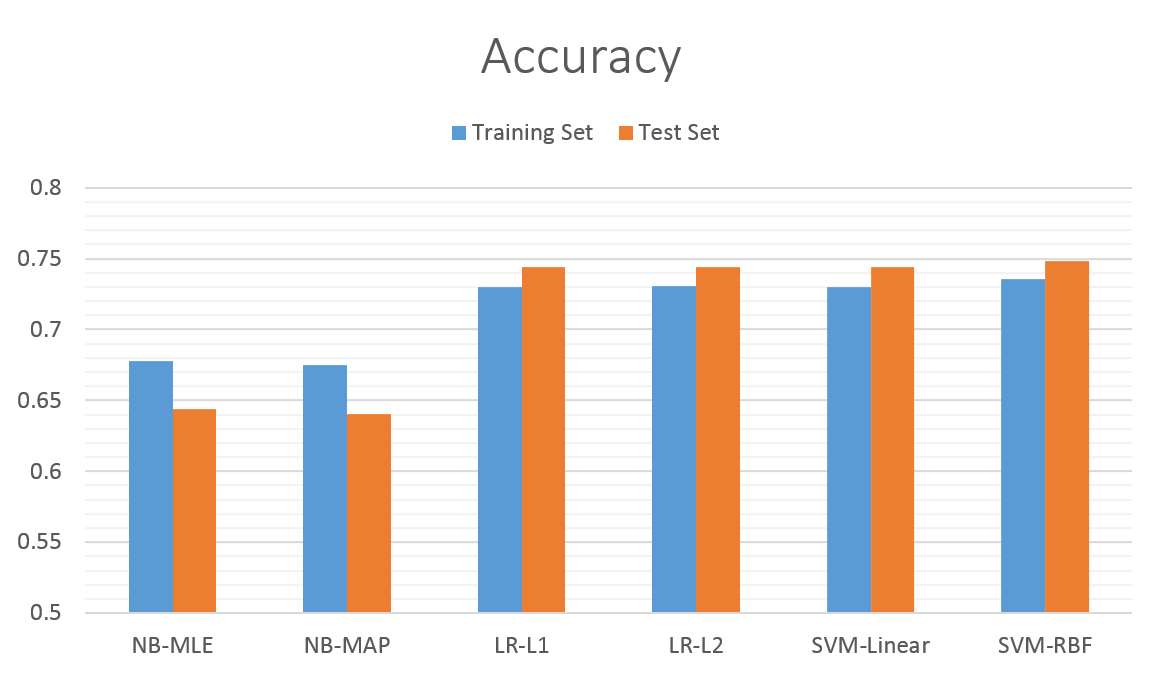
\includegraphics[scale=0.4]{Accuracy.png}
\end{center}
\caption{Accuracy of different classifiers}
\end{figure}


\begin{figure}[H]
\begin{center}
%\framebox[4.0in]{$\;$}
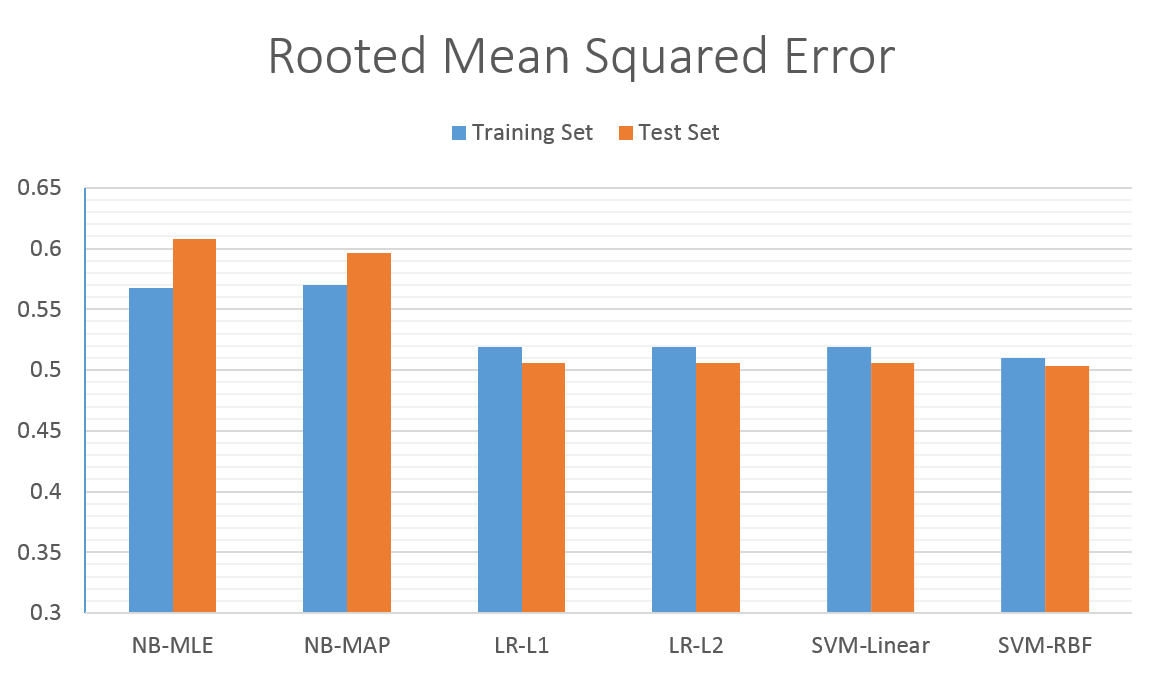
\includegraphics[scale=0.4]{RMSE.png}
\end{center}
\caption{RMSE of different classifiers}
\end{figure}


 
Naive Bayes classifier can be done in linear time, but it generates very high RMSE. The features in this problem are not conditional independent, however, Naive Bayes has a strong requirement that each feature is conditional dependent with each other. When applying AdaBoost to Naive Bayes, the result is greatly improved, but still not high enough. So Naive Bayes may not be an ideal classifier for this problem.

For Logistic Regression and linear SVM, the time complexity is also relativly low. Compared to Naive Bayes, the classification result of Logistic Regression is much better. However, the accuracy of our LR and linear SVM classifier is still not high. 

For non-linear SVM, the time complexity is very high. The result is similar to the result of linear SVM. Expending our features to a higher dimension can still not improve the performance.


\iffalse
\begin{figure}[H]
\begin{center}
\begin{minipage}[h]{0.4\linewidth}
\centering
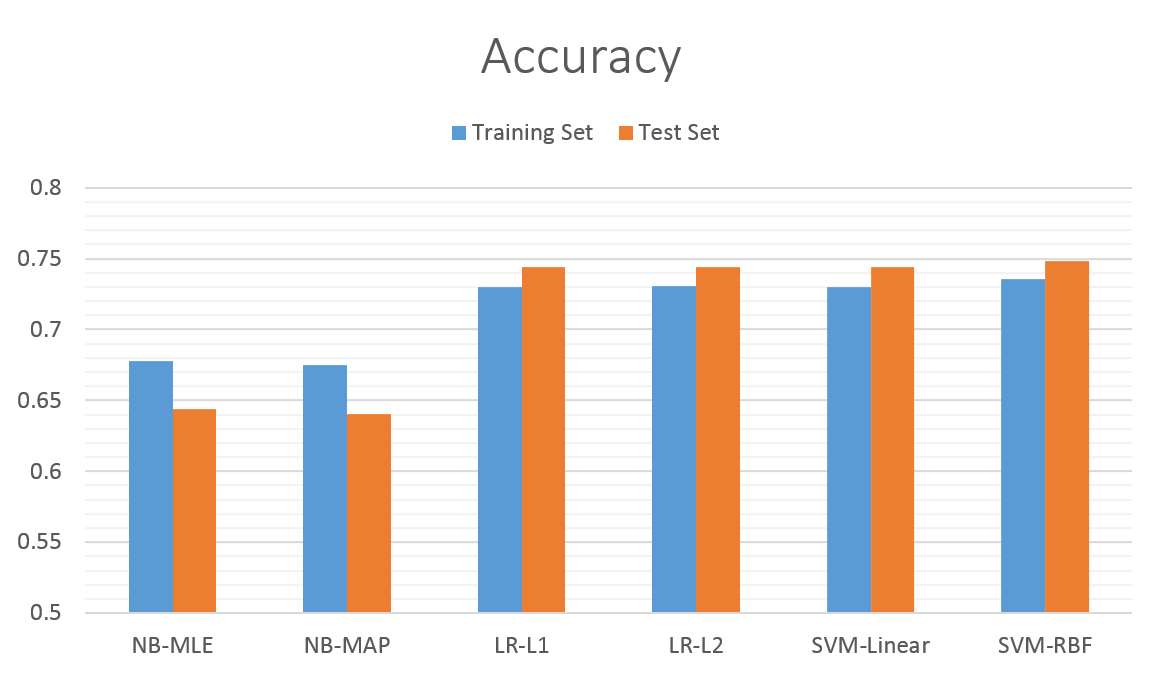
\includegraphics[width=1\textwidth]{Accuracy.png}
\caption{Accuracy of different classifiers}
\label{skyline}
\end{minipage}
\begin{minipage}[h]{0.4\linewidth}
\centering
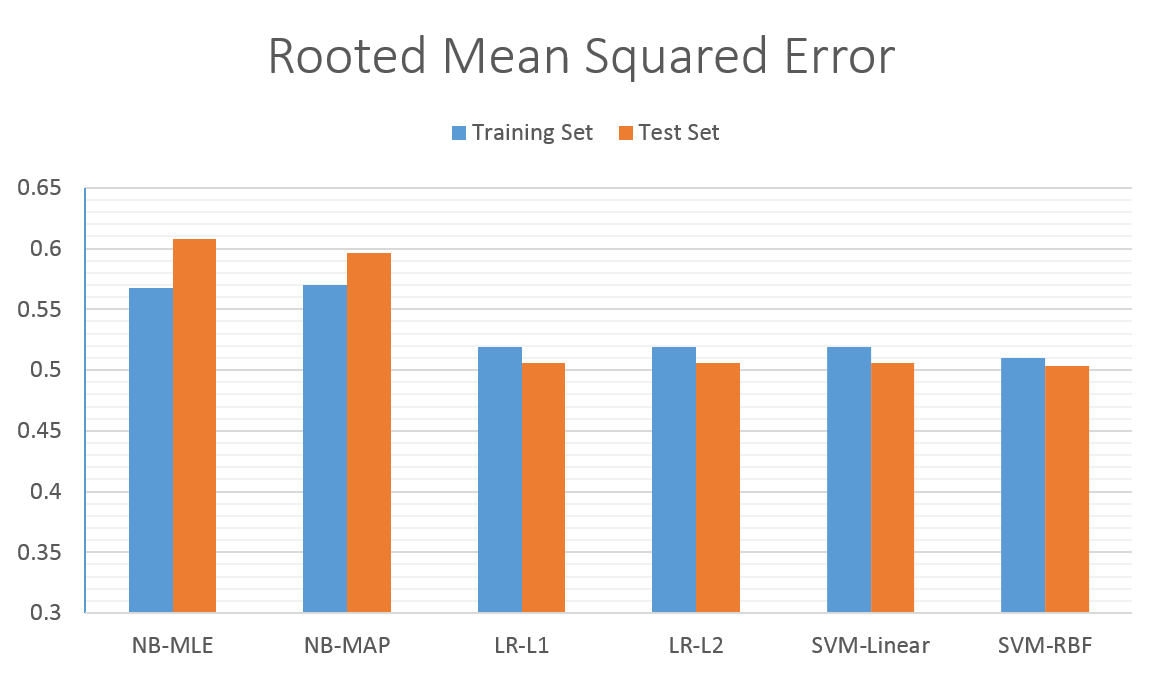
\includegraphics[width=1\textwidth]{RMSE.png}
\caption{RMSE of different classifiers}
\label{skyline}
\end{minipage}
\end{center}
\end{figure}
\fi


\section{Next Step}
On the next step, we will focus more on feature extraction. The best result we get for now will be chosen as the new benchmark in the next step. Our target will still be to improve the predicting accuracy as well as decreasing the RSME.

Specifically, here are the steps that we plan to try:
\begin{itemize}
\item Use larger dataset to train each classifier.
\item Assemble more features not limited to the given columns to increase feature diversity.
\item Add student temporal learning information to the feature vector. For example, for each step, add step name and Knowledge Component from the previous few steps. In addition, we can also record whether a student has met a problem or knowledge component before.
\end{itemize}

\subsubsection*{References}
\small{
[1] Pardos Z A, Gowda S M, Baker R S J, et al. The sum is greater than the parts: ensembling models of student knowledge in educational software[J]. ACM SIGKDD explorations newsletter, 2012, 13(2): 37-44.

[2] Yu H F, Lo H Y, Hsieh H P, et al. Feature Engineering and Classifier Ensemble for KDD Cup 2010[J].

[3] Zach A. Pardos, neil T.Heffernan. Using HMMs and bagged decision trees to leverage rich features of user and schoolroom an intelligent tutoring system dataset. 

[4] Andreas T\"{o}scher, Michael Jahrer. Collaborative Filtering Applied to Educational Data Mining.

[5] Fan, Rong-En, et al. "LIBLINEAR: A library for large linear classification." The Journal of Machine Learning Research 9 (2008): 1871-1874.

[6] Chang, Chih-Chung, and Chih-Jen Lin. "LIBSVM: a library for support vector machines." ACM Transactions on Intelligent Systems and Technology (TIST) 2.3 (2011): 27.


}

\end{document}
